\chapter{Implementation}\label{ch4}

\section{Technology Stack}
Table~\ref{ch4:tab-stack} summarises the production stack used in the CryptoVolt repository. The backend is intentionally monolithic inside a single FastAPI application for clarity during research; the frontend is a single-page application built with Vite for fast iteration.

\begin{table}[ht]
\centering
\caption{Major technologies in the implemented system.}
\label{ch4:tab-stack}
\resizebox{0.98\linewidth}{!}{%
\begin{tabular}{@{}llp{6.8cm}@{}}
\toprule
\textbf{Layer} & \textbf{Technology} & \textbf{Role} \\
\midrule
API & Python 3, FastAPI, Uvicorn & REST endpoints, OpenAPI docs, CORS, lifespan hooks \\
Persistence & SQLAlchemy, SQLite or PostgreSQL & Users, sessions, trading records; \texttt{DATABASE\_URL} selects backend \\
ML & XGBoost, PyTorch, scikit-learn, pandas, NumPy & Training jobs, inference, metrics \\
NLP & VADER, PRAW (Reddit) & Sentiment scoring and optional social ingestion \\
Charts / TA & \texttt{ta}, Recharts (frontend) & Indicators and dashboard candles \\
Client UI & React 18, TypeScript, Vite & Dashboard, auth flow, API proxy in dev \\
\bottomrule
\end{tabular}%
}
\end{table}

\section{Backend Organisation}
Routers are grouped under \texttt{/api} prefixes: \texttt{auth}, \texttt{coins}, \texttt{market}, \texttt{sentiment}, \texttt{trading}, \texttt{paper}, \texttt{ml}, \texttt{backtest}, and \texttt{alerts}. Shared dependencies include a database session provider and JWT validation for protected routes. Environment variables are loaded from the repository root \texttt{.env} for local runs.

\section{Market and Sentiment Services}
Klines are retrieved through Binance-compatible service modules and exposed to the dashboard for symbol and interval selection. Sentiment endpoints aggregate text-derived scores; when Reddit credentials are configured, additional posts can inform training or live windows.

\section{Machine Learning Training Pipeline}
Training is triggered via the ML API (e.g.\ XGBoost multi-symbol jobs). Jobs run asynchronously: the client receives a job identifier and polls status. Completed runs write artefacts into a configurable model registry directory on disk and may emit metrics or dataset exports under \texttt{\_datasets/} for audit.

\section{Hybrid Trading and Paper Trading}
The trading router exposes a decision endpoint that combines model outputs with rule-based logic; a veto flag and human-readable reason are returned to the UI. Paper trading routes maintain simulated positions without placing real exchange orders, enabling safe experimentation.

\section{Frontend Dashboard}
The dashboard page loads recommended symbols, fetches klines for charting, and displays sentiment and hybrid decisions. Figure~\ref{ch4:fig-ui} shows a representative layout of the live interface (styling may vary by theme).

\begin{figure}[ht]
\centering
\begin{tikzpicture}
\node[draw=sibau-sea-green!80!black, line width=1pt, rounded corners=3mm, fill=sibau-sea-green!6, inner sep=2pt] {%
  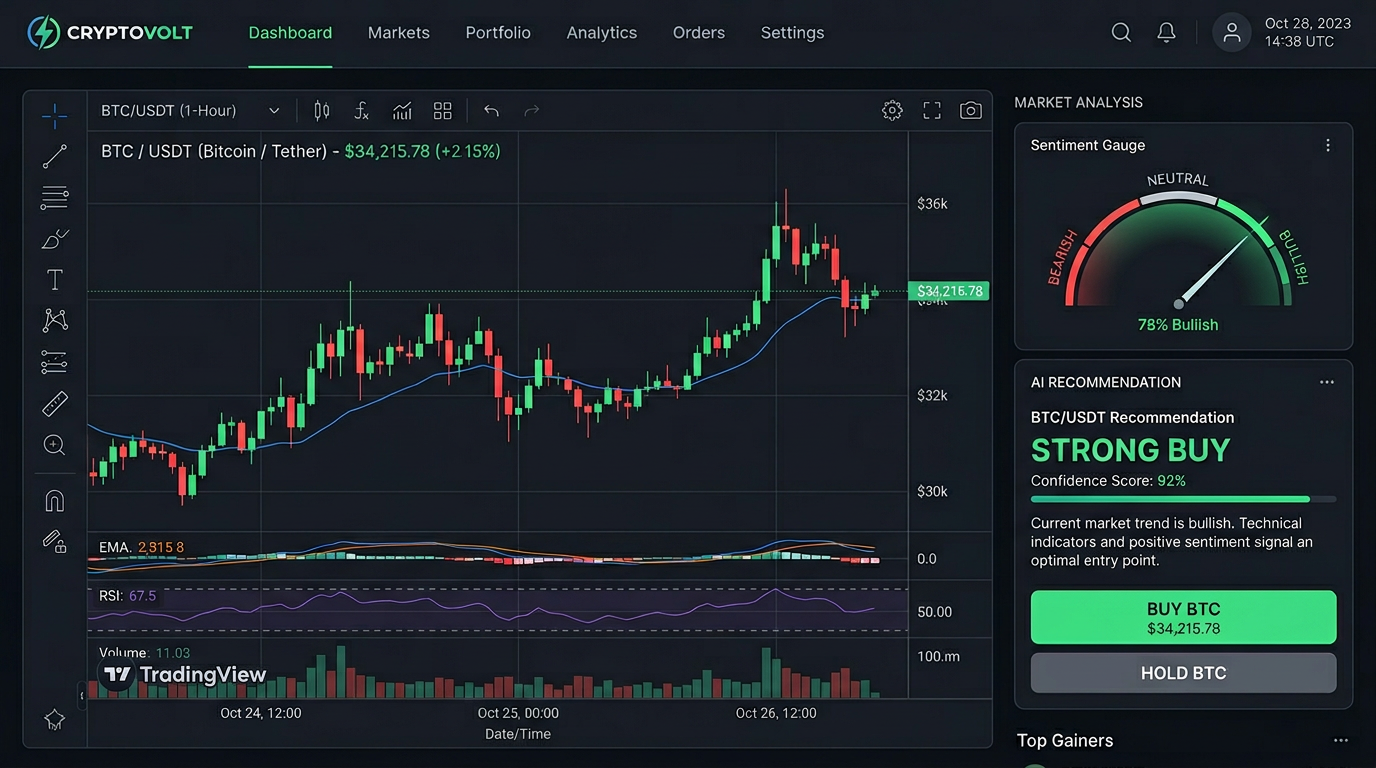
\includegraphics[width=0.92\linewidth]{figures/dashboard-ui}%
};
\end{tikzpicture}
\caption{Representative CryptoVolt dashboard view: market chart, sentiment summary, and trading decision panel.}
\label{ch4:fig-ui}
\end{figure}

\section{Alerting}
Discord webhooks and in-app alert records (where implemented) notify operators of notable events or test messages. Configuration is via environment variables to avoid hard-coding secrets.

\section{API Documentation and Developer Experience}
FastAPI automatically exposes an OpenAPI schema and interactive documentation (typically at \texttt{/docs}) so that endpoints, request bodies, and response models can be explored without reading source code. Figure~\ref{ch4:fig-openapi} shows a representative documentation view; the exact layout depends on the browser and FastAPI version.

\begin{figure}[ht]
\centering
\begin{tikzpicture}
\node[draw=sibau-sky-blue!70!black, line width=1pt, rounded corners=3mm, fill=sibau-sky-blue!6, inner sep=2pt] {%
  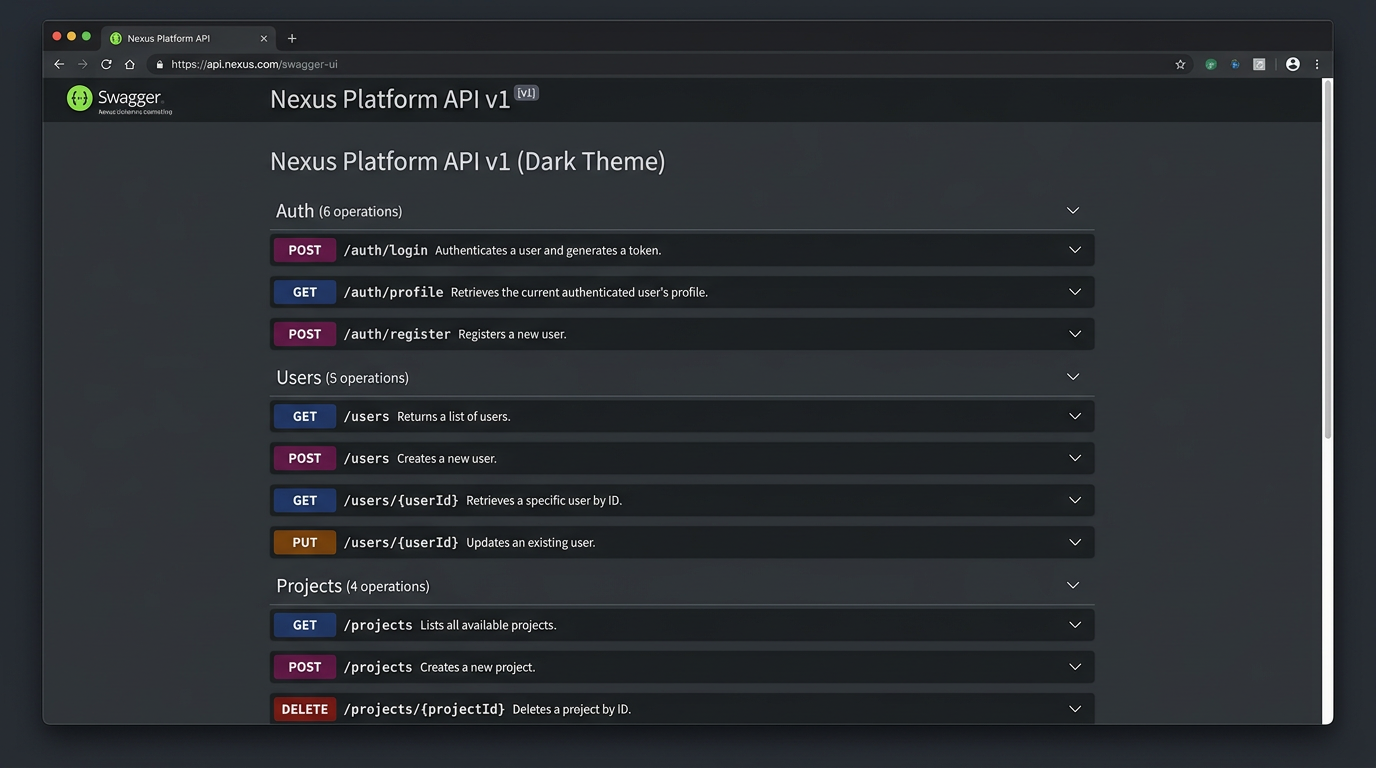
\includegraphics[width=0.92\linewidth]{figures/openapi-docs-ui}%
};
\end{tikzpicture}
\caption{Interactive API documentation (Swagger-style) generated from the FastAPI application.}
\label{ch4:fig-openapi}
\end{figure}

\section{Module Interaction}
Figure~\ref{ch4:fig1} depicts how browser, API, and persistence layers interact during a typical authenticated dashboard request.

\begin{figure}[ht]
\centering
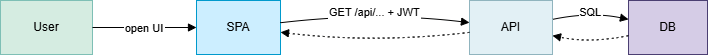
\includegraphics[width=0.96\linewidth]{figures/figure-4-4-custom}
\caption{Simplified request path for an authenticated dashboard call (not to scale).}
\label{ch4:fig1}
\end{figure}
